\section{Fretbord}

\subsection{Notennamen}

\begin{minipage}[b]{0.48\textwidth}
Elk vakje op de gitaar heeft een bepaalde toonhoogte. Deze vakjes, of preciezer gezegd, de metalen strips, heten de fretten.

Als iemand bijvoorbeeld vraagt om de 2e fret op de 3e snaar in te drukken, dan zet je je vinger op het groene puntje in \ref{fig:ukulele_string_fretting}.
\end{minipage}
\hfill
\begin{minipage}{0.48\textwidth}
    \centering
    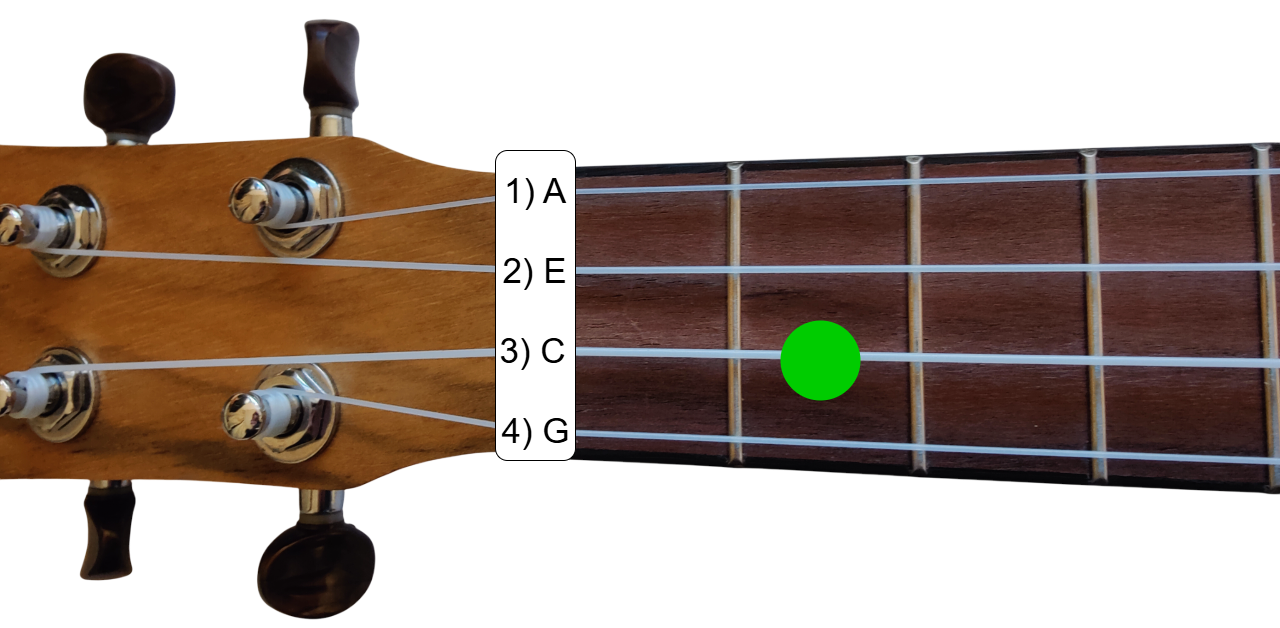
\includegraphics[width=\textwidth]{../Images/ukulele-neck-fretting.png}
    \captionof{figure}{Het groene puntje is de 2e fret op de 3e snaar}
    \label{fig:ukulele_string_fretting}
\end{minipage}

Zoals eerder gezegd heeft elke fret heeft een eigen toonhoogte. In de muziek zijn er 12 verschillende tonen die in verschillende octaven (hier komen we later op terug) gespeeld kunnen worden. De namen van deze tonen zie je hieronder.

\begin{table}[h]
\centering
\begin{tabular}{*{12}{P{5mm}}}
\large{A} & \large{A$\sharp$} & \large{B} & \large{C} & \large{C$\sharp$} & \large{D} & \large{D$\sharp$} & \large{E} & \large{F} & \large{F$\sharp$} & \large{G} & \large{G$\sharp$}
\end{tabular}
\end{table}

Je ziet dat er maar \textbf{7} verschillende letters zijn, en \textbf{5} letters met een \textbf{$\sharp$}. Deze $\sharp$ symbolen heten \textbf{kruizen}. Een kruis wil zeggen dat de toon één fret omhoog gaat. Een stap van één fret wordt ook wel een halve stap genoemd.

%\infobox{De reden dat er kruizen worden gebruikt en niet de noten A, B, C, D, E, F, G, H, I, J, K, L, heeft de maken met de geschiedenis van de muziek.}

In \ref{fig:ukulele_single_string_octave_sharps} zijn de noten in een C octaaf te zien. In the TAB is te zien op welke fret en op welke snaar dat op de ukulele gespeeld wordt. In \ref{fig:ukulele_multi_string_octave_sharps} zijn dezelfde noten te zien, maar dan gespeeld op andere snaren (zie de TAB).

\begin{figure}[h]
    \centering
    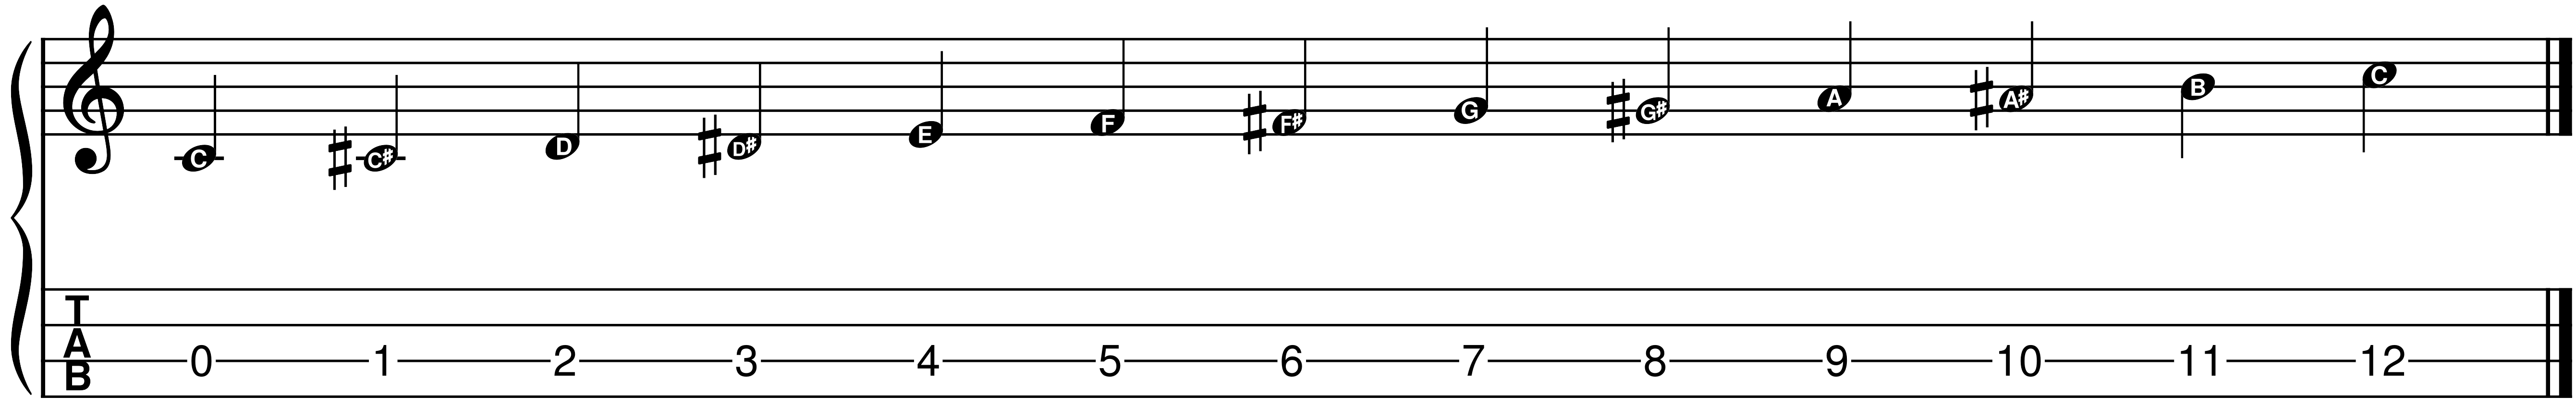
\includegraphics[width=\textwidth]{../MuseScore/Ukulele/UkuleleChromaticNotesSharpsSingleString.png}
    \caption{Een octaaf van C naar C op de 3e C snaar met kruizen}
    \label{fig:ukulele_single_string_octave_sharps}
\end{figure}

\begin{figure}[h]
    \centering
    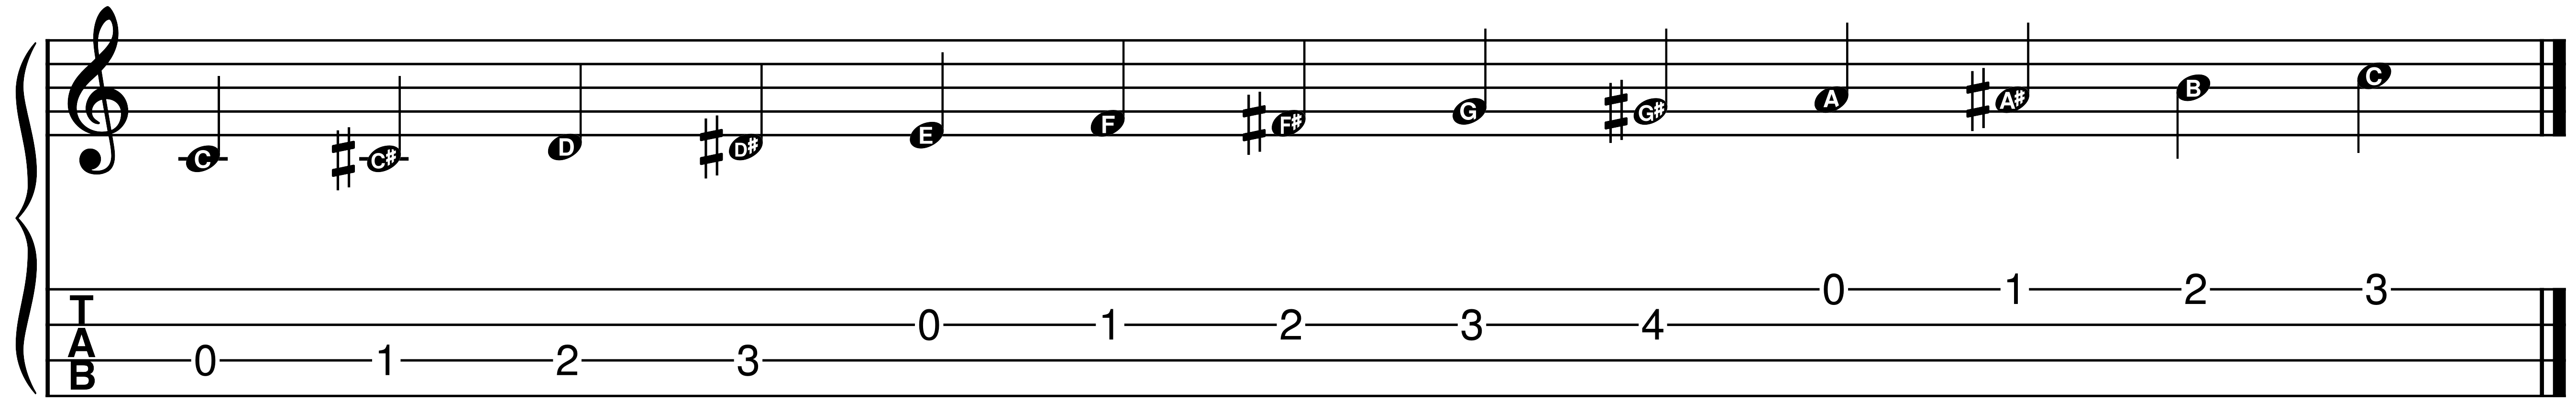
\includegraphics[width=\textwidth]{../MuseScore/Ukulele/UkuleleChromaticNotesSharpsMultiString.png}
    \caption{Een octaaf van C naar C op de snaren 1 t/m 3 met kruizen}
    \label{fig:ukulele_multi_string_octave_sharps}
\end{figure}

\newpage

Ter referentie kan \ref{fig:ukulele_fretboard_filled} gebruikt worden om een noot op het fretbord te vinden. Probeer nu echter niet meteen alle noten te onthouden. Dit zal vanzelf gaan tijdens latere oefeningen.

\begin{figure}[h]
    \centering
    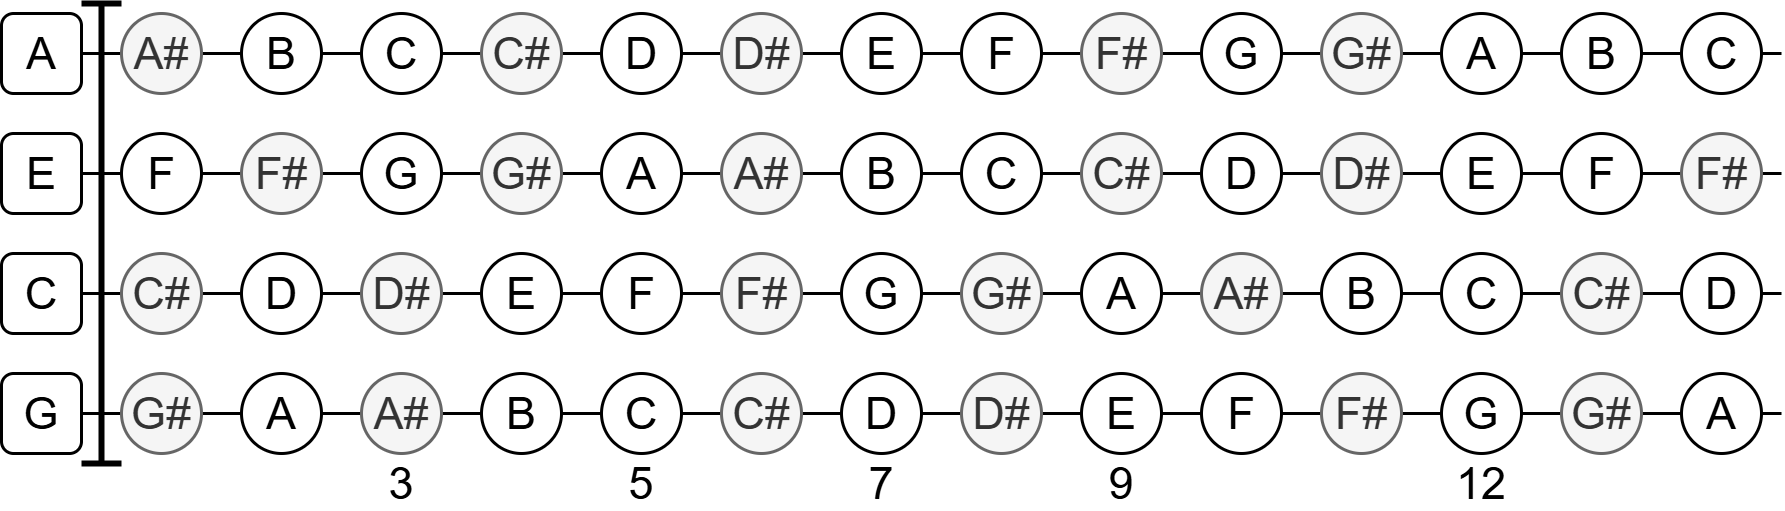
\includegraphics[width=\textwidth]{../Images/Fretboard-Ukulele-filled.png}
    \caption{Alle noten op ukulele gestemd met GCEA}
    \label{fig:ukulele_fretboard_filled}
\end{figure}

Naast kruizen zijn er ook mollen. Een mol ($\flat$) wil zeggen dat de noot één fret (een halve stap) omlaag gaat. Als je \ref{fig:ukulele_multi_string_octave_sharps} dus met mollen zou schrijven in plaats van kruizen krijg je \ref{fig:ukulele_fretboard_filled_flats}.

In \ref{fig:ukulele_fretboard_filled_flats} zie je ook het nieuwe herstel teken ($\natural$). Dit wil zeggen dat de noot waarvoor een $\flat$ of $\sharp$ was gezet, nu weer 'normaal' is. Als er namelijk een $\flat$ of $\sharp$ bij een noot is gezet, geldt dit voor alle noten met dezelfde naam voor de rest van de maat. Wat een 'maat' is komen we zo op.

\begin{figure}[h]
    \centering
    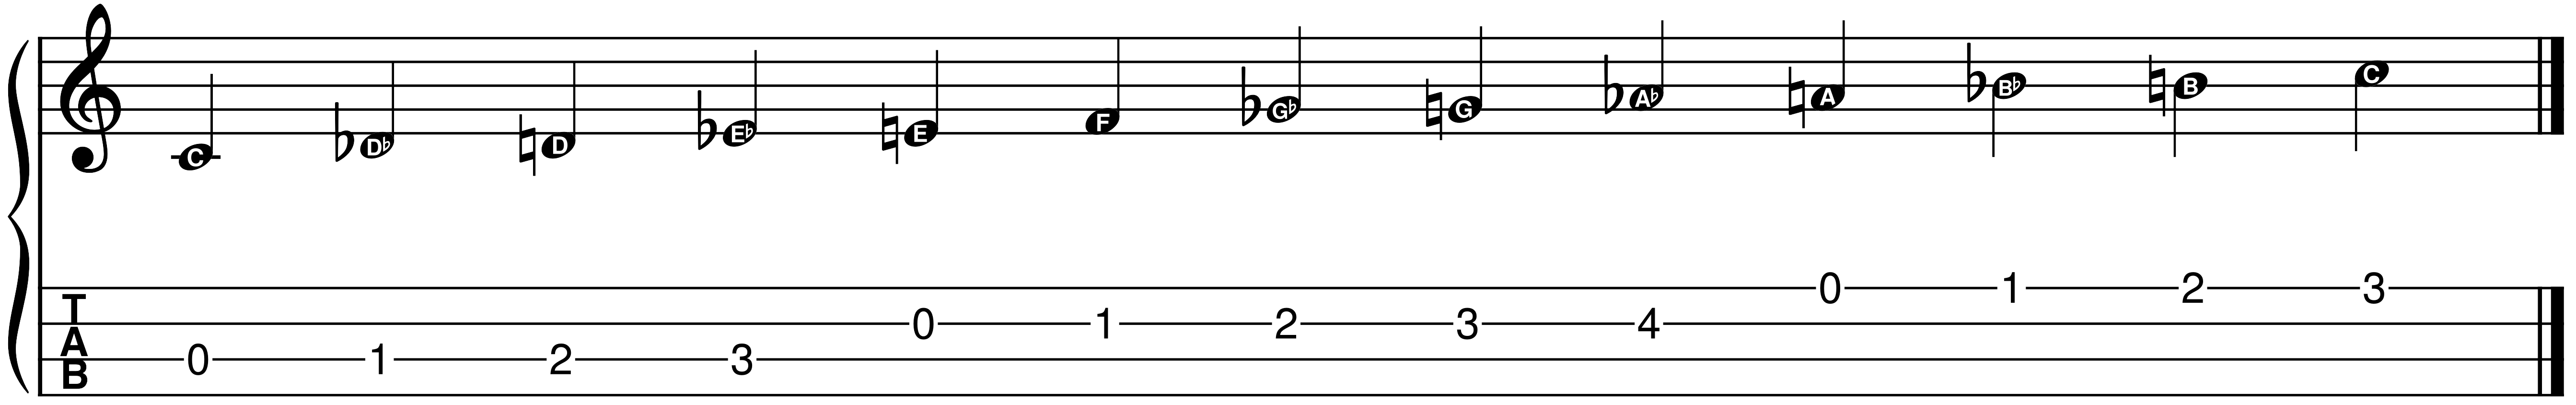
\includegraphics[width=\textwidth]{../MuseScore/Ukulele/UkuleleChromaticNotesFlatsMultiString.png}
    \caption{Een octaaf van C naar C op de snaren 1 t/m 3 met mollen en herstel symbolen}
    \label{fig:ukulele_fretboard_filled_flats}
\end{figure}

TODO: Things about measures, treble clef, names of the of notes on the score, etc.

\newpage

\subsection{Tonische noten}

\begin{minipage}{0.48\textwidth}
Eerder hebben we de ukulele gestemd met een stemapparaat. Dit moet je natuurlijk altijd doen. Maar naast dat de snaren de juiste toonhoogte hebben, is het net zo van belang dat de noten relatief aan elkaar de juiste toonafstand hebben. De toonafstand tussen noten is namelijk wat er voor zorgt dat noten wel of niet mooi samen klinken.

In \ref{fig:ukulele_tonic_intervals} zien je welke twee fretten (het interval) dezelfde toonhoogte hebben. Dus als je wilt kijken of de 3e C snaar en 2e E snaar de juiste toonafstand hebben, dan kan je je vinger op de 4e fret op C snaar zetten, en de E snaar open aanspelen. dit zou dezelfde toonhoogte moeten hebbben. Zo niet, dan kan je aan de stemknop draaien tot het goed klinkt.

Vergelijke \ref{fig:ukulele_fretboard_filled} en \ref{fig:ukulele_tonic_intervals} maar eens. Dan zul je zien dat de groene punten dezelfde nootnaam hebben.

Om de snaren op elkaar af te stemmen worden de volgende combinaties gebruikt:

\begin{itemize}
    \item[\textbf{A}] Fret 5 snaar 2 - open snaar 1
    \item[\textbf{E}] Fret 4 snaar 3 - open snaar 2
    \item[\textbf{C}] Dit is al de laagste toon
    \item[\textbf{G}] Fret 3 snaar 2 - open snaar 4
\end{itemize}

\end{minipage}
\hfill
\begin{minipage}{0.35\textwidth}
    \centering
    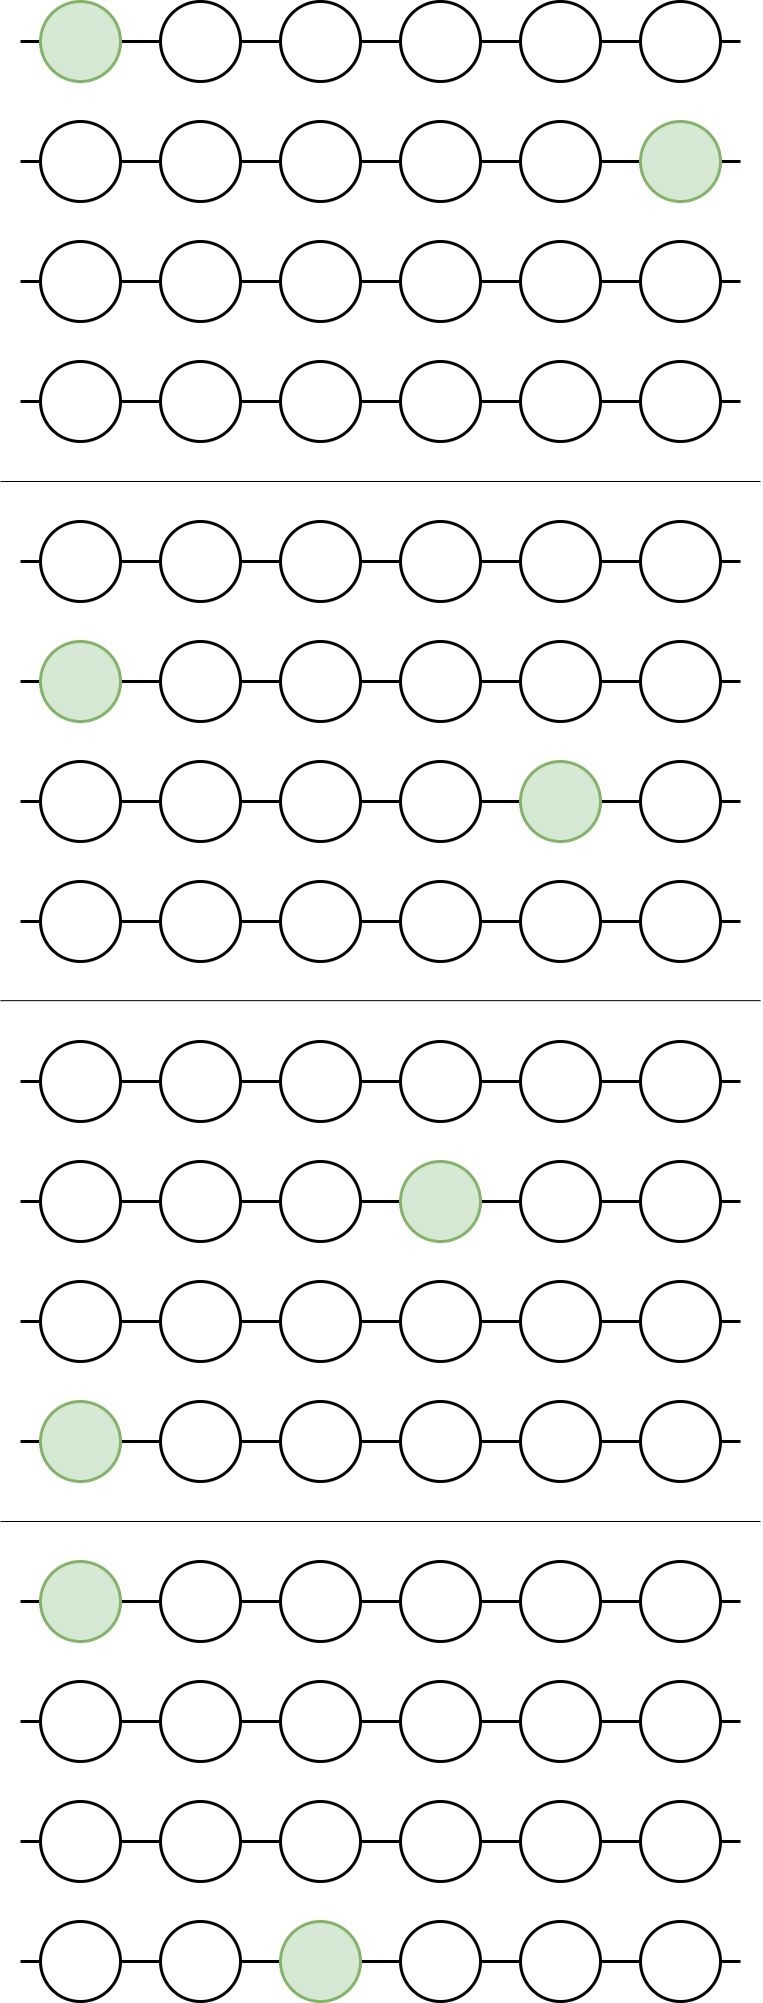
\includegraphics[width=\textwidth]{../Images/ukulele-fretboard-tonics.png}
    \captionof{figure}{Tonische intervallen op de ukulele}
    \label{fig:ukulele_tonic_intervals}
\end{minipage}

\newpage

\subsection{Octaven}

Er zijn ook octaven te vinden op de ukulele. Deze zijn te zien in \ref{fig:ukulele_octave_intervals}. Waar de toonhoogte bij de vorige intervallen hetzelfde was, zijn ze hier een octaaf van elkaar af.

Weten waar de octaven liggen is handig wanneer er meer over de toonladders geleerd wordt.

\begin{figure}[h]
    \centering
    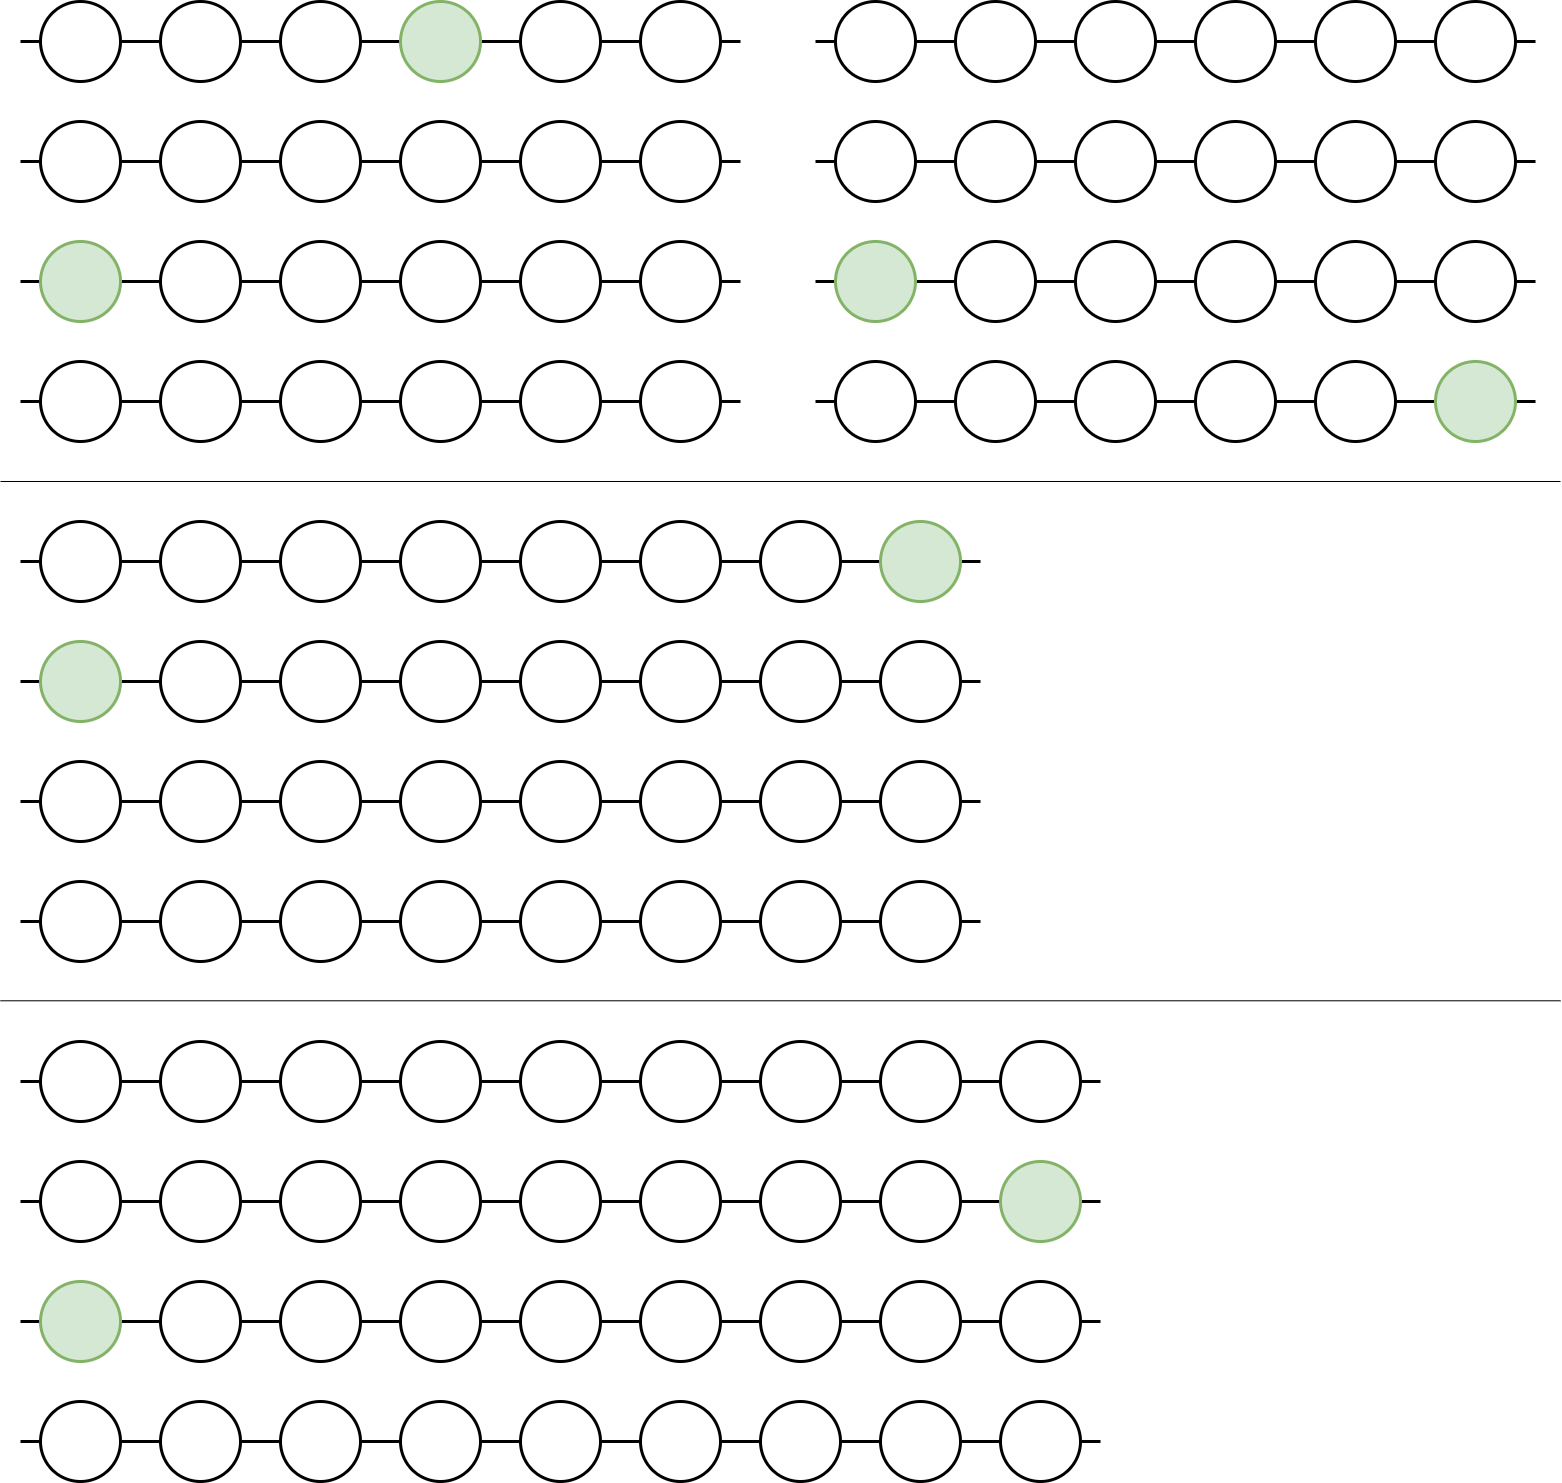
\includegraphics[width=0.75\textwidth]{../Images/ukulele-fretboard-octaves.png}
    \captionof{figure}{Octaaf intervallen op de ukulele}
    \label{fig:ukulele_octave_intervals}
\end{figure}

